\clearpage
\section{Normal SPI with continuously enabled MISO: 15 November 2026}
Temporary image \texttt{1cf28c8f} adds retained output-enable control to the
previous diagnostic, keeping LVCMOS33 DRIVE12/SLEW SLOW, the original SPI
parser and the DD29/cable path. CSR 0x306 mode 0 retains HSEL-controlled
Hi-Z; mode 4 changes only the output enable to always active, leaving raw
parser data unchanged even at idle; mode 5 additionally forces data zero
outside HSEL. Parser hold and explicit MISO clamp remain disabled throughout.
The same configured image is used for every comparison; there is no reload
or external clock reconfiguration between modes.

Observer format 0x30004 adds the logical output-enable source at bit 13.
This verifies commanded behavior in sampled logic, not electrical pad voltage.
Simulation of the actual generated routing expressions with the original
parser verified read0/1/2 replies, idle Hi-Z, continuous enable, idle-data
selection and return to normal mode. Dell timing passed with setup slack
0.062 ns and hold slack 0.071 ns.

The ordered primary blocks are A0, B4, A0, C5, A0, B4, A0, all read0/divider601.
Each block includes an idle capture. Functional checks in modes4/5 use reads
0/1/2 at dividers601/61, followed by normal-mode controls. Mode changes settle
for50ms before arming; their transients outside these windows are not measured.
Generator/observer share MCLK1 and retain the common-reference-stop limitation.

The first run stopped after one positive SPI control because a repeated
write of unchanged parser mode0 timed out following SYS reset. Partial raw
records and executed source were retained, and original-image restoration,
power/frontend and physical ADC checks passed. The repeated wrapper removes
that no-op write and verifies parser mode by bounded readback instead.

\subsection{Completed write-only comparison}
The original MCU DMA command recognizer uses sync bytes
\texttt{78 56 34 12 98 BA DC FE} or eight AA bytes for reset.
The local adapter permits only scratch address0x40 with fixed values
0000, FFFF, 5555 and 0F0F; these exact packets contain none of the sync/reset
bytes. The global shared-bus read-only allowlist is retained. The reference
hash, exact packets and qualification basis are archived. No real peripheral
control register is written.

Three write-only blocks use normal MISO, explicit MISO0 clamp, then normal
MISO again. Each value is written three times. Scratch value and write-counter
increment are verified through IPbus303/304, without any SPI readback.
All36 writes committed correctly. The parser remains active in all three
blocks. A write frame does not imply quiet MISO: the diagnostic parser's
shift register drives MISO even while receiving a write.

\begin{center}\begin{tabular}{lrrr}\toprule
Written value & Normal MISO & MISO clamped0 & Normal return\\\midrule
0000 &1/3&0/3&2/3\\
FFFF &3/3&0/3&3/3\\
5555 &2/3&0/3&3/3\\
0F0F &2/3&0/3&3/3\\\midrule
Total SYS reset/LOCK losses &8/12&0/12&11/12\\\bottomrule
\end{tabular}\end{center}
Pure SPI writes can therefore reproduce the failure. In this ordered series,
forcing MISO0 suppressed it while preserving write acceptance; restoring normal
MISO reproduced it. This strengthens the association with MISO activity during
SPI but does not identify electrical coupling or exclude phase/pattern effects.

\begin{center}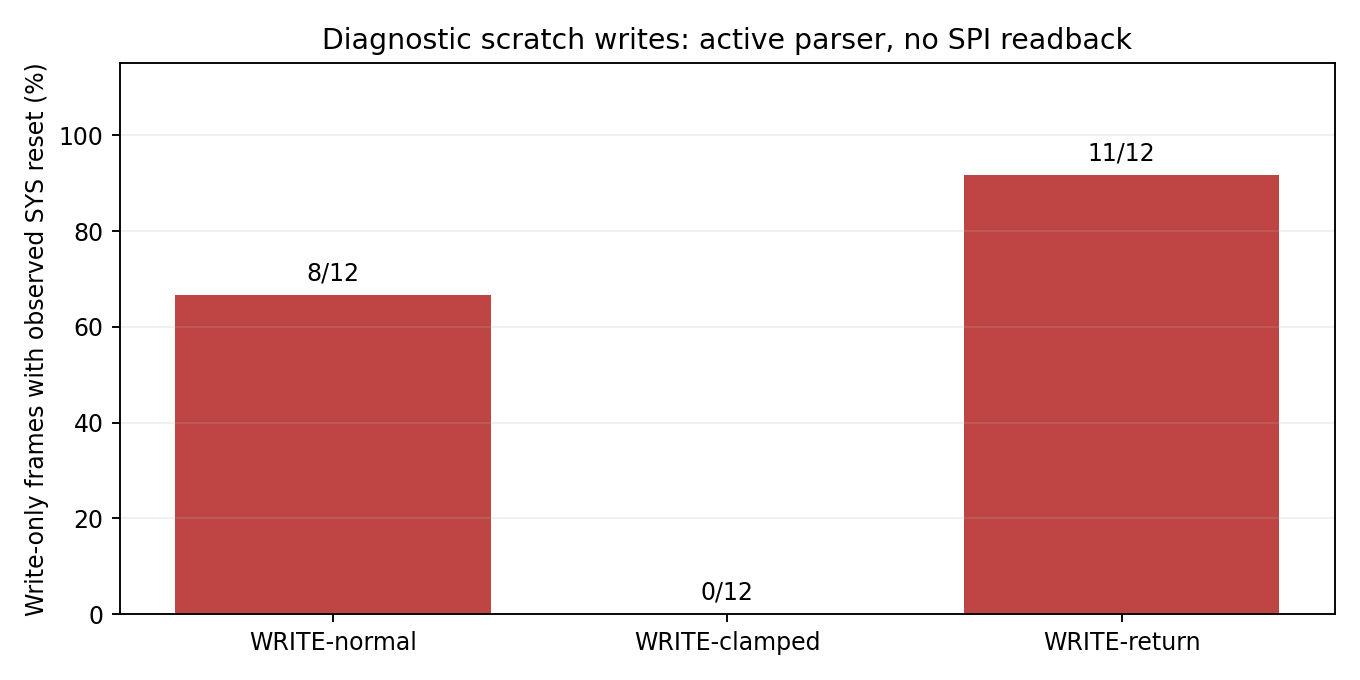
\includegraphics[width=\linewidth]{spi-writes.png}\end{center}
\subsection{Output-enable result and transport limitations}
After the write blocks, normal read0/div601 gave6/6 resets, continuously enabled
MISO with unchanged raw data gave6/6, and normal return gave6/6. All signatures
were correct. Sampled OE matched the commanded behavior, including all idle
samples. Removing Hi-Z therefore did not suppress the fault in this comparison;
Hi-Z transitions are not necessary for reproduction.

The larger planned OE campaign was not completed. Earlier cohorts stopped
on a no-op write timeout or lost ARM commands after repeated SYS resets;
partial runs remain separate. The final run uses a fresh IPbus UDP socket per
window and bounded generation-checked ARM retries. Its36-write series and
A0/B4/A0 blocks completed, but mode5 (additional zero outside SEL) was not
confirmed by register readback, so that window is unmeasured and not counted.
The wrapper exits with an error after that failed mode change; the completed
measurements are not represented as a successful full protocol.

\begin{center}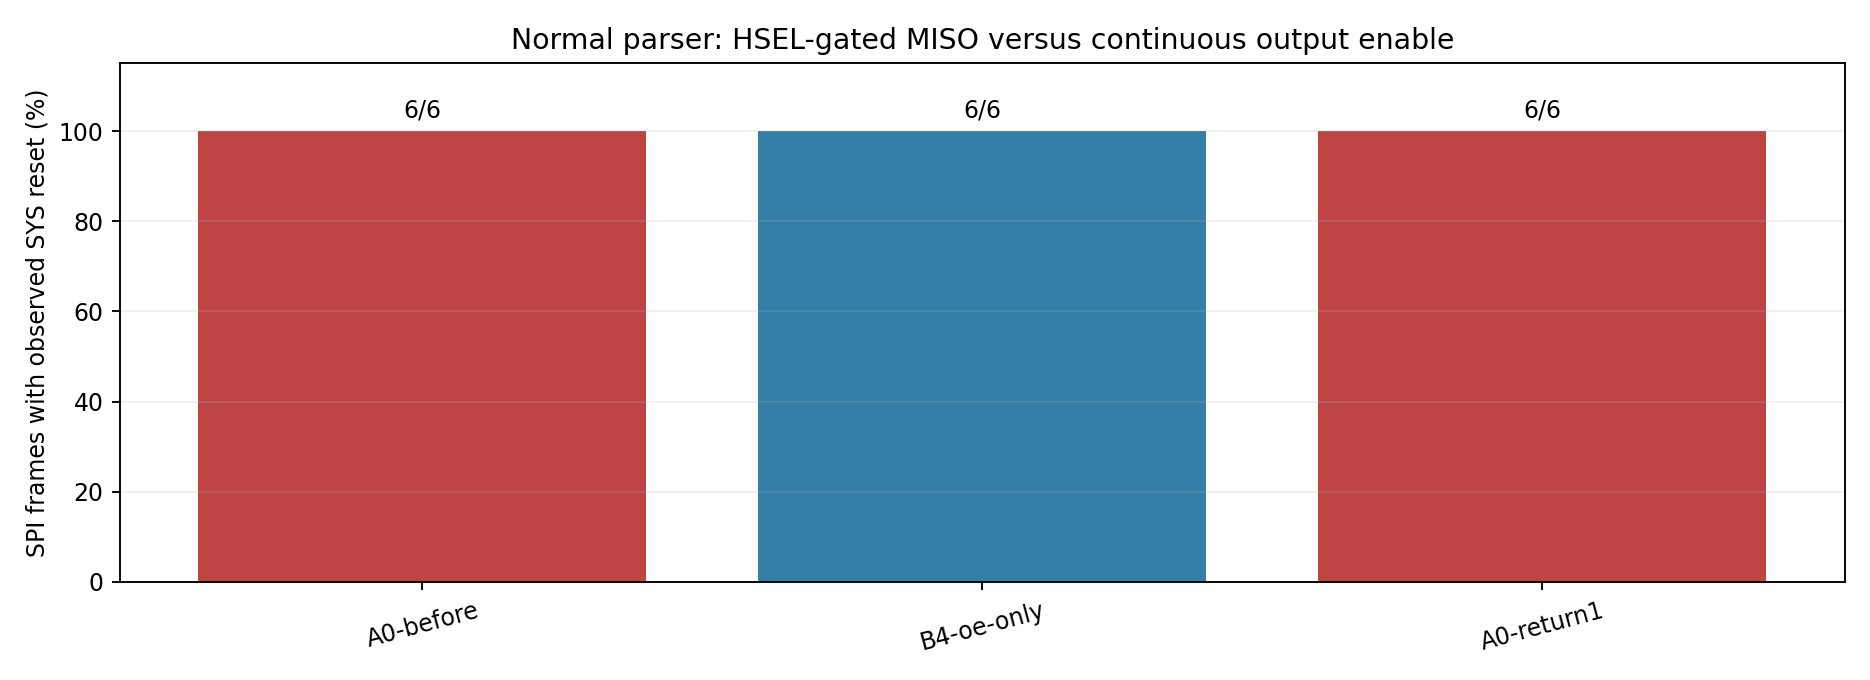
\includegraphics[width=\linewidth]{miso-oe.png}\end{center}
\begin{center}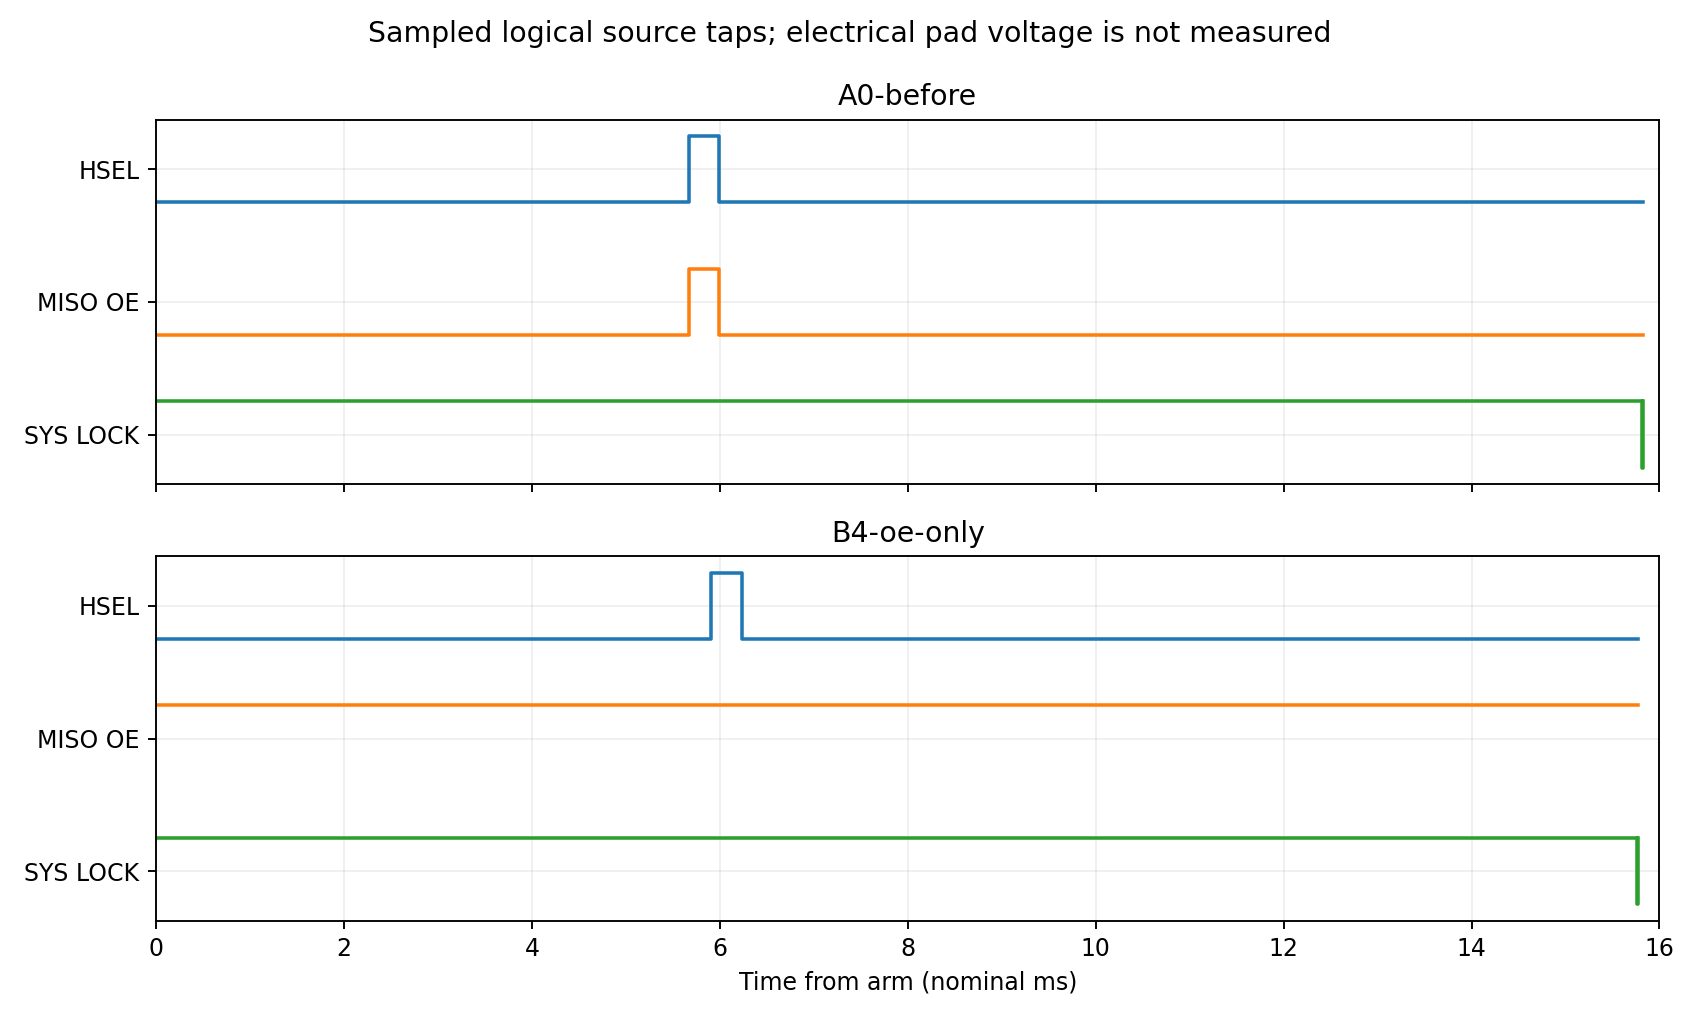
\includegraphics[width=\linewidth]{miso-oe-traces.png}\end{center}
For quiet timed windows, plots extend the last unchanged logical state to the
known timed freeze. They are not electrical waveform measurements.

Exact originalc7531465 was restored after every run. The final power/frontend
checks passed (frontend0xfff), and all12 physical ADC bank-A captures passed
on the first attempt. Kasli outputs stayed driven and its divider was restored.
Raw/partial captures, executed wrappers, source/bitstream, simulations, qualified
Dell reports and restoration receipts are archived in:
\begin{center}\path{system/evidence-miso-oe-20261115}\end{center}
